\documentclass{article}
\usepackage[margin=1in]{geometry}
\usepackage{amsmath,amsfonts,amssymb}
\usepackage{listings}
\usepackage{color}
\usepackage{graphicx}
\usepackage{subfig}
\usepackage{blkarray}
\usepackage{multirow}
\usepackage{float}
\usepackage{caption}
\usepackage{subcaption}
\begin{document}
\begin{titlepage}
	\setlength{\parindent}{0pt}
	\large

\vspace*{-2cm}

\definecolor{dkgreen}{rgb}{0,0.6,0}
\definecolor{gray}{rgb}{0.5,0.5,0.5}
\definecolor{mauve}{rgb}{0.58,0,0.82}

\lstset{frame=tb,
  language=Python,
  aboveskip=3mm,
  belowskip=3mm,
  showstringspaces=false,
  columns=flexible,
  basicstyle={\small\ttfamily},
  numbers=none,
  numberstyle=\tiny\color{gray},
  keywordstyle=\color{blue},
  commentstyle=\color{dkgreen},
  stringstyle=\color{mauve},
  breaklines=true,
  breakatwhitespace=true,
  tabsize=3
}

University of Waterloo \par
CS 480 \par
\vspace{0.05cm}
r2knowle: 2023-11-28
\vspace{0.2cm}

{\huge Exercise \# 3 \par}
\hrule

\vspace{0.5cm}
\textbf{Q3a)} For this question, we will be using our VG11 NN trained for the last assignment. The test accuracy is $98.99\%$ and the model summary is:
\begin{lstlisting}
Model: "sequential"
_________________________________________________________________
 Layer (type)                Output Shape              Param #   
=================================================================
 conv2d (Conv2D)             (None, 32, 32, 64)        640                                  
 batch_normalization         (None, 32, 32, 64)        256       
 (BatchNormalization)                                                                                        
 max_pooling2d               (None, 16, 16, 64)        0         
 (MaxPooling2D)                                                                                                                          
 conv2d_1 (Conv2D)           (None, 16, 16, 128)       73856                                                              
 batch_normalization_1       (None, 16, 16, 128)       512       
 (BatchNormalization)                                                                                                        
 max_pooling2d_1             (None, 8, 8, 128)         0         
 (MaxPooling2D)                                                                                                                    
 conv2d_2 (Conv2D)           (None, 8, 8, 256)         295168                                                          
 batch_normalization_2       (None, 8, 8, 256)         1024      
 (BatchNormalization)                                                    
 conv2d_3 (Conv2D)           (None, 8, 8, 256)         590080                                                            
 batch_normalization_3       (None, 8, 8, 256)         1024      
 (BatchNormalization)                                                                                                 
 max_pooling2d_2             (None, 4, 4, 256)         0         
 (MaxPooling2D)                                                            
 conv2d_4 (Conv2D)           (None, 4, 4, 512)         1180160                                                        
 batch_normalization_4       (None, 4, 4, 512)         2048      
 (BatchNormalization)                                                                                                            
 conv2d_5 (Conv2D)           (None, 4, 4, 512)         2359808                                                        
 batch_normalization_5       (None, 4, 4, 512)         2048      
 (BatchNormalization)                                                                                                       
 max_pooling2d_3             (None, 2, 2, 512)         0         
 (MaxPooling2D)                                                                                                                   
 conv2d_6 (Conv2D)           (None, 2, 2, 512)         2359808                                                     
 batch_normalization_6       (None, 2, 2, 512)         2048      
 (BatchNormalization)
 conv2d_7 (Conv2D)           (None, 2, 2, 512)         2359808                                                            
 batch_normalization_7       (None, 2, 2, 512)         2048      
 (BatchNormalization)                                                                                                         
 max_pooling2d_4             (None, 1, 1, 512)         0         
 (MaxPooling2D)                                                                                                                      
 flatten (Flatten)           (None, 512)               0                                                               
 dense (Dense)               (None, 4096)              2101248                                                               
 dropout (Dropout)           (None, 4096)              0                                                                 
 dense_1 (Dense)             (None, 4096)              16781312                                                           
 dropout_1 (Dropout)         (None, 4096)              0                                                            
 dense_2 (Dense)             (None, 10)                40970     
                                                                 
=================================================================
Total params: 28153866 (107.40 MB)
Trainable params: 28148362 (107.38 MB)
Non-trainable params: 5504 (21.50 KB)
_________________________________________________________________
\end{lstlisting}
\newpage
\textbf{Q3b)} Below are 15 samples of test images for the 3 degrees of epsilon in FGSM adversary training. The first row denotes $\epsilon = 0.1$, the middle row denotes $\epsilon = 0.2$ and finally the last row denotes $\epsilon = 0.5$:
\begin{center}
\includegraphics[width=.8\linewidth]{q3bFGSM.png}
\end{center}
We can observe that as epsilon increases the amount of noise in the images increases. The background intensity will always increase, and the pixels of the actual digit tend to decrease. At epsilon 0.5 it means the perturbed parts of the digit are indistinguishable from the perturbed parts of the background. \\

With our base model we receive the following test accuracies for the perturbed test set:
\begin{center}
\begin{tabular}{||c | c |c ||} 
 \hline
 Test Accuracy on $ \epsilon = 0.1$ & Test Accuracy on $ \epsilon = 0.2$ & Test Accuracy on $ \epsilon = 0.5$ \\ [0.5ex] 
 \hline
 $59.95\%$ & $31.63\%$ & $15.58\%$ \\ 
 \hline
\end{tabular}
\end{center}
As should be expected we see that as epsilon increase the training accuracy decreases.  \\

\textbf{Q3c)} After doing adversarial training (one generated image per training image) we get the following test accuracies:

\begin{center}
\begin{tabular}{|c | c |c |} 
 \hline
 Test Accuracy on $ \epsilon = 0.1$ & Test Accuracy on $ \epsilon = 0.2$ & Test Accuracy on $ \epsilon = 0.5$ \\ [0.5ex] 
 \hline
 $97.04\%$ & $91.18\%$ & $80.32\%$ \\ 
 \hline
\end{tabular}
\end{center}
After doing adversarial training we can see that our model accuracies increase by a very large extent. We also notice that expect of epsilon 0.2, that as epsilon increase our model accuracy decreases proportionately. 
\newpage
\textbf{Q3d)} Below are 15 samples of test images for the 3 degrees of epsilon in PGD adversary training. The first row denotes $\epsilon = 0.1$, the middle row denotes $\epsilon = 0.2$ and finally the last row denotes $\epsilon = 0.5$: 
\begin{center}
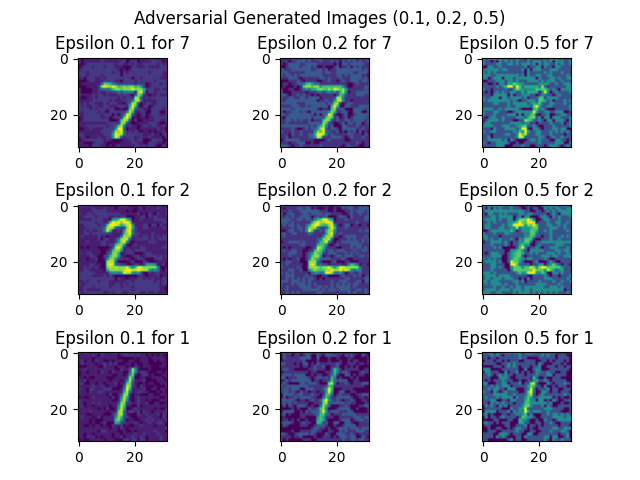
\includegraphics[width=.8\linewidth]{q3bPGD.png}
\end{center}
Below are the three tables comparing the 3 different trained models versus the three different test sets:
\begin{center}
\begin{tabular}{| c || c | c | c |} 
 \hline
Model Type & Unperturbed Test Set  & FGSM Test Set & PGD Test set\\ [0.5ex] 
 \hline
 Untrained & $98.37\%$ & $59.94\%$ & $77.81\%$ \\ 
 \hline
 FGSM & $74.12\%$ & $97.04\%$ & $86.07\%$ \\ 
 \hline
 PGD & $73.10\%$ & $99.07\%$ & $98.07\%$ \\ 
 \hline
\end{tabular}
\captionof{table}{Test Accuracies for $\epsilon = 0.1$}
\end{center}
\begin{center}
\begin{tabular}{| c || c | c | c |} 
 \hline
Model Type & Unperturbed Test Set  & FGSM Test Set & PGD Test set\\ [0.5ex] 
 \hline
 Untrained & $98.37\%$ & $31.63\%$ & $33.65\%$ \\ 
 \hline
 FGSM & $74.12\%$ & $99.18\%$ & $89.23\%$ \\ 
 \hline
 PGD & $73.10\%$ & $97.54\%$ & $96.68\%$ \\ 
 \hline
\end{tabular}
\captionof{table}{Test Accuracies for $\epsilon = 0.2$}
\end{center}
\begin{center}
\begin{tabular}{| c || c | c | c |} 
 \hline
Model Type & Unperturbed Test Set  & FGSM Test Set & PGD Test set\\ [0.5ex] 
 \hline
 Untrained & $98.37\%$ & $15.58\%$ & $9.36\%$ \\ 
 \hline
 FGSM & $74.12\%$ & $80.32\%$ & $61.23\%$ \\ 
 \hline
 PGD & $73.10\%$ & $62.23\%$ & $87.38\%$ \\ 
 \hline
\end{tabular}
\captionof{table}{Test Accuracies for $\epsilon = 0.5$}
\end{center}
Note that both FGSM and PGD were trained with an $epsilon = 0.2$. From this we can identify some trends. The first is that as epsilon increases, each model tends to do worse on tests that they were note trained on. The untrained model's accuracy falls off far faster on adversary tests and then adversarial trained models do on normal data. We also notice that the model trained on PGD data tends to be more robust and has higher accuracy on FGSM data then the FGSM model has on PGD data. Lastly we notice that each model has around $~98\%$ accuracy on the data it was trained on.
\end{titlepage}
\end{document}